% \newpage
% \chapter{Other models tested}

\section{M3: Document embedding by averaging word-vectors}

We initially tried a basic scenario where documents are represented by a fixed length vector which can then be used for classification even though each document can be of a different length.

One of the common techniques to generate new embeddings to documents is by using an existing pre-trained word embeddings by averaging the word vectors to create a single fixed size embedding vector.

\begin{figure}[htbp]
\centering
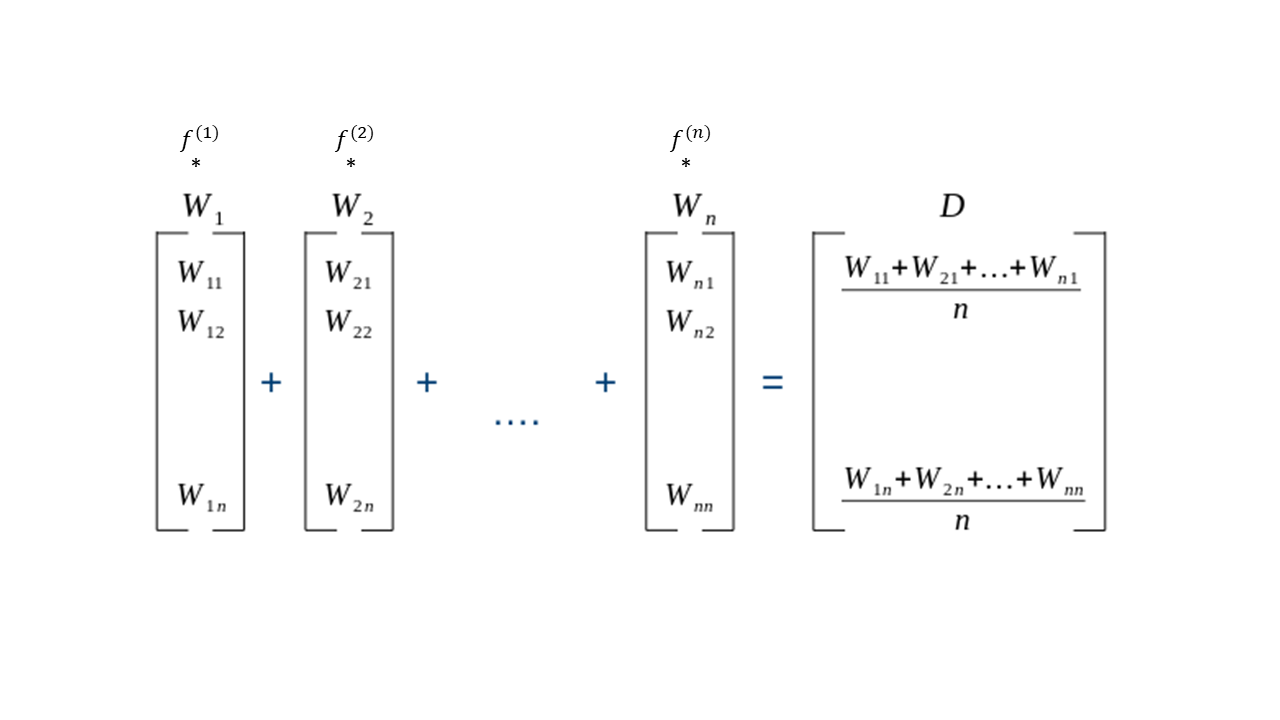
\includegraphics[width=16cm, height=8cm]{images/average-vectors.png}\\
\centering
\caption{Average word-vectors}
\label{fig:foo}
\end{figure}

\subsection{Steps to compute fixed embedding vector}

\begin{itemize}
\item {First we import a word vector model that either has been pre-trained by Google or retrained on the training data to obtain domain specific word vectors.}
\item {Then we iterate over the entire corpus and generate a mean vector for each document.}
\end{itemize}
Once we obtain the mean vector for all the documents, we train a vanilla logistic regression model using the thus generated fixed embedding feature matrix.

\begin{figure}[htbp]
\centering
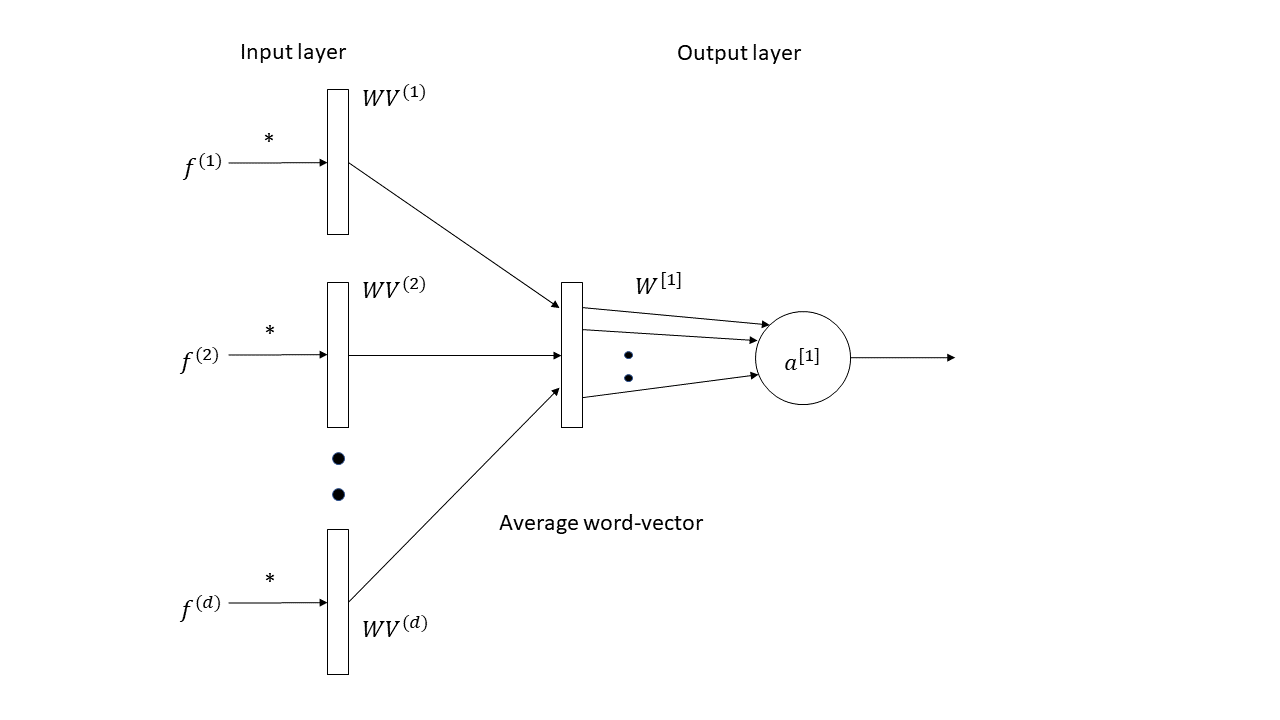
\includegraphics[width=16cm, height=8cm]{images/average-vectors2.png}\\
\centering
\caption{Average word-vectors model}
\label{fig:foo}
\end{figure}

% \newpage
% \section{Initial word-vector model}
%
% For our initial word-vector model, we built a network where the coefficients are only a function of its word representation ($v^{(i)}$), without the logistic regression weights, i.e.,
%
% \begin{equation}\label{lb1}
% \theta^{(i)} = \theta_{wv}^{(i)}
% \end{equation}
%
% These weights as mentioned in Chapter 3, will be learnt through the word representation of the features using a linear regressor, which will then be passed through a sigmoid/softmax function for classfication i.e.,
%
% \begin{equation}
% \theta_{wv}^{(i)} = w_{1}v_{1}^{(i)} + w_{2}v_{2}^{(i)} + ... + w_{d}v_{d}^{(i)} = \sum_{d=1}^{D} w_{d}^{(i)}v_{d}^{(i)}
% \end{equation}
%
% where, $w = (w_{1}, w_{2}, ..., w_{d})$ are the parameters of the regression function.
%
% $\quad\qquad\  v= (v_{1}, v_{2}, ..., v_{d})$ are d-dimensional word-representations of word $i$\\
%
% \textbf{Comparison with CNN}
%
% If we compare the word-vector coefficients model to a CNN, then this would be similar to a 1D CNN network having one filter, sum pooling and a sigmoid/softmax activation function at the output layer with cross entropy loss. We are training on a bag-of-words model which does not consider the order of the sentence, so the kernel size which decides the length of the 1d convolutional window would be 1. Also, from our network we can see that the coefficients are a linear sum of the word-vector representation with no activation layer at the end. To replicate the same on the CNN network, we do not apply an activation function to the single filter. It is directly passed onto the sum pooling layer. This network would then be like the word vector coefficients model.
%
% If our task is multi-class classification, then the model can be seen as a CNN model with N filters and softmax function as the activation function, where N equals to the number of the classes in the dataset. We should change the sum pooling layer to make them work in a "filter-wise" style, which means you want to sum over features from the same filter. After pooling layer, the shape of the output should be N*1, where N is the number of filters.
%
% If our task is multi-label classification, everything is the same as the multi-class setup except the activation function is sigmoid.
%
% \begin{figure}[htbp]
% \centering
% 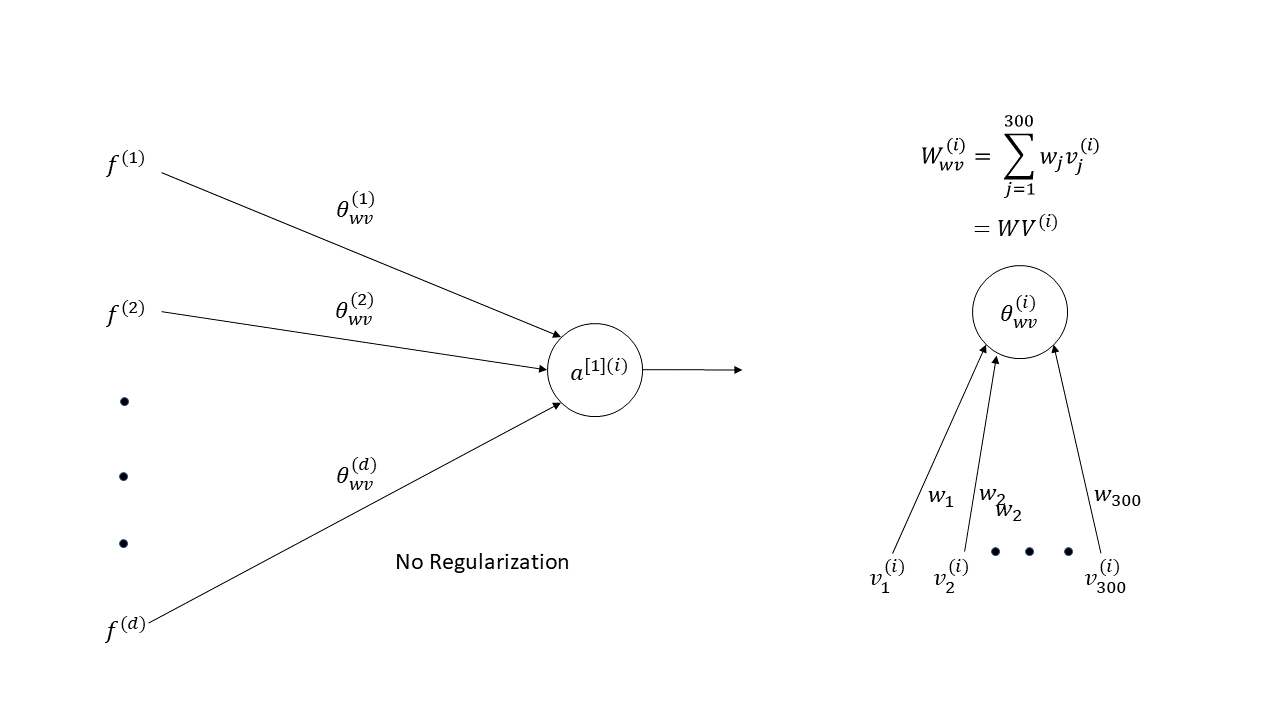
\includegraphics[width=16cm, height=8cm]{images/init-wv.png}\\
% \centering
% \caption{Initial word-vectors model}
% \label{fig:foo}
% \end{figure}
%
% \begin{figure}[htbp]
% \centering
% 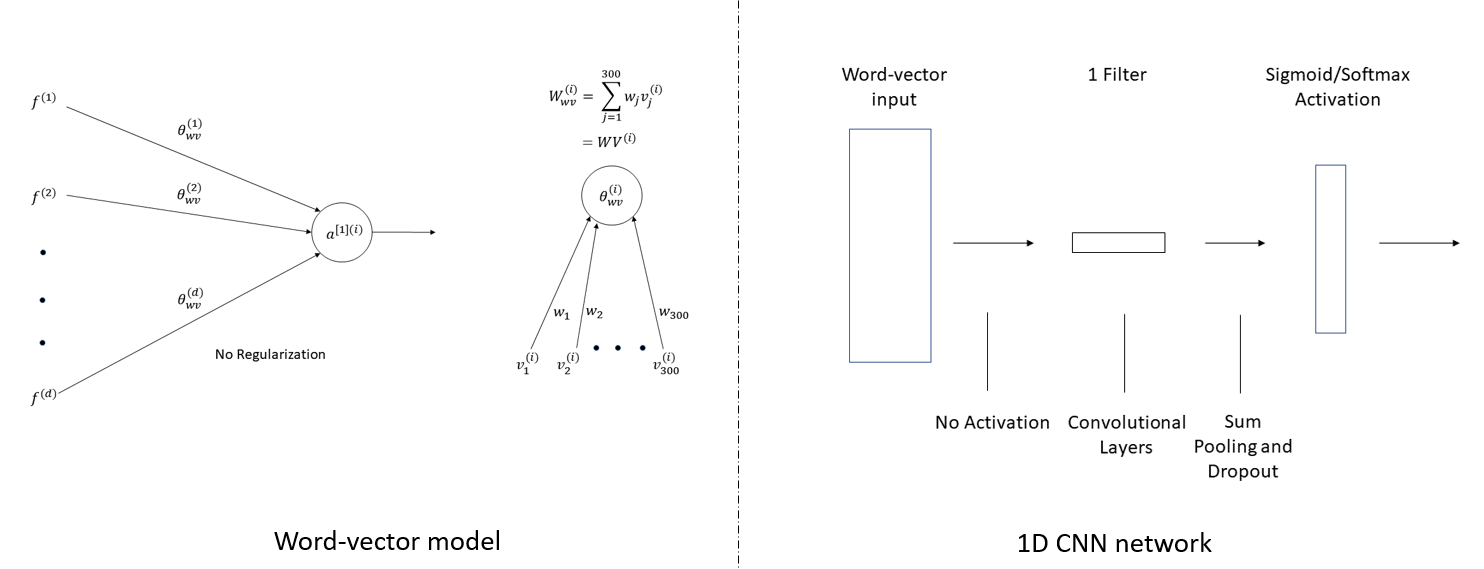
\includegraphics[width=16cm, height=8cm]{images/wv-cnn.png}\\
% \centering
% \caption{Comparison of word-vector with CNN model}
% \label{fig:foo}
% \end{figure}

% \newpage
\section{M4: Vanilla logistic regression with word-vector regularization}

Our proposed method trained a model using coefficients trained from both the vanilla logistic regression model and word-vectors. In this model, instead of generating the feature weights using the word-vectors, we use the word-vectors as a regularizer that is added to the cost function. This regularizer would add a higher penalty to similar words having large differences in their corresponding feature weights. This kind of regularization should technically enforce similar words to have similar weights.

Thus, similar to logistic regression the probability the class variable $y_{j}=1, j=1,2,...m$ can be modelled as follows:

\begin{equation}
\ P(y_{j}  = 1 | x_{j}; \theta) = h_{\theta}(x_{j}) = \frac{1}{1+e^{-\theta^{T}x_{(j)}}}
\end{equation}

Using the principle of maximum likelihood estimate, we find the parameters that maximize the likelihood P(X $|$ y). Hence the log-likelihood is given as,

\begin{equation}
\ L(\theta) = \sum_{i=1}^{m}{y_{i}log(h_{\theta}(x_{i})) + (1-y_{i})log(1-h_{\theta}(x_{i}))}
\end{equation}

Maximizing the log-likelihood is similar to minimizing -L($\theta$) over all data points. The cost function for the logistic regression model comes out to be,

\begin{equation}
\ J(\theta) = -\frac{1}{m}{L(\theta)}
\end{equation}

Adding L1, L2 and word-vector regularization to this we get:

\begin{equation}
\ J(\theta) = -\frac{1}{m}{L(\theta)} + \frac{\lambda_{1}}{m}{|{\theta}|} + \frac{\lambda_{2}}{m}{|{\theta}|}^{2} + 
\frac{\lambda_{3}}{m}{(WV Reg)}
\end{equation}

where $\lambda_{1}, \lambda_{2}, \lambda_{3}$ and l1, l2 and word-vector regularization constraints.\\

\noindent Given a dataset of $n$ features, we compute the word-vector regularization as follows:

\begin{itemize}
\item Compute the cosine similarity between all feature's words-vectors. This will give us a $(n$ x $n)$ dimensional similarity matrix
\item Compute the difference between the corresponding feature weights $\theta$. This will also give us an $(n$ x $n)$ dimensional matrix that contains the difference between a feature's weight to all other weights
\item Perform a matrix multiplication between the similarity matrix and the matrix having the difference between the coefficients
\item The final result will act as a word-vector regularizer which can be added to the overall cost function regularized by a regularization parameter $\lambda_{3}$

\end{itemize}

\begin{figure}[htbp]
\centering
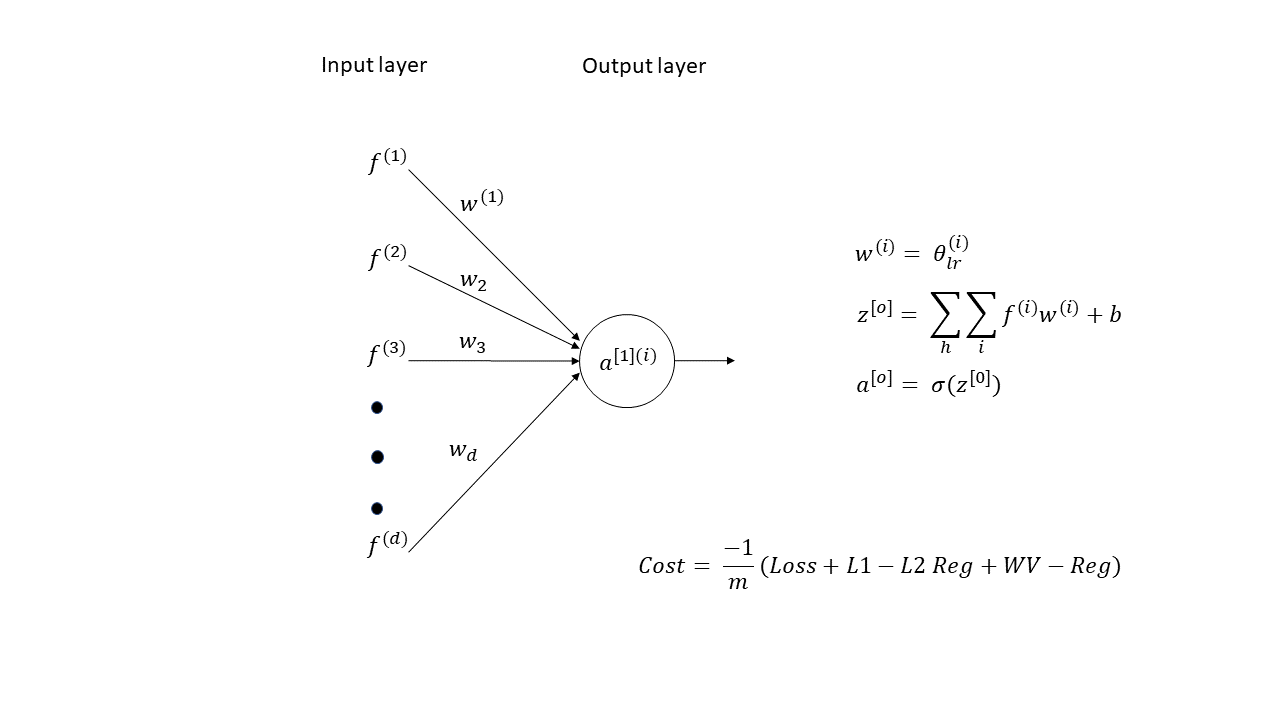
\includegraphics[width=16cm, height=10cm]{images/model3.png}\\
\centering
\caption{Logistic Regression with Word-vector regularization}
\label{fig:foo}
\end{figure}

% \newpage
\textbf{Why would it work?}
Let's say there are two words "Russia" and "Soviet" having similar word-vectors due to their reference in similar context. However the word "Russia" is present in the text more often than "Soviet" and has higher feature weight. Due to their high similarity and larger difference in weights, the word-vector model will add a higher penalty to the cost function until their corresponding weights are close to each other.

Now the claim is that the cost function would be minimized if the word-vector penalty is minimum. Now let's think about a few cases: 

\begin{itemize}
    \item \textbf{Case 1:} If two features $x_{i}$, $x_{j}$ are completely dissimilar, their cosine similarity is 0, and they don't contribute to the cost function
    \item \textbf{Case 2:} If two features are completely alike, their cosine similarity is 1. Now we have two subcases:
    \begin{itemize}
        \item \textbf{Subcase 1:} Both features have similar weights, thus the difference between their weights is 0. This would also not contribute to the cost function.
        
        \item \textbf{Subcase 2:} Both features have very different weights, thus the difference between their weights would be large. This would \textit{increase} the overall cost function. This is precisely the examples we are looking for: similar features having very different weights. So the algorithm forces them to have the same weights.
    \end{itemize}
\end{itemize}

\subsection{Challenges faced}

The major challenge faced while running this model is the amount of time it took to generate the weight differences matrix and computing its dot product with the similarity matrix. Since the model was trained using mini-batch gradient descent, we had to compute the word-vector regularization cost at the end of every mini-batch in order to update the weights. 

So for a medium sized dataset with 10,000 features, 100,000 records and a decent batch size of 10\% of training data, one would have to compute these matrices and get their dot product at least 10 times. And that would train the model for just a single epoch. For training a good enough model with a decent learning rate, one would need to train the model for at least 400-500 epochs. All of this only if we are training a binary classifier. If we are training a multi-class or multi-label classifier with $\sim$2000 different classes, then it would take an exponential amount of time. This puts a huge constraint on the amount of time and resources needed to train the model. For training an even larger dataset with $\sim$100,000 features, it would be even more difficult as training a single epoch itself might take a few hours.

\subsection{Workarounds}

In order to remediate this, we limit the features for which we want to increase the weights. Since our objective through this project was to make rare features have higher weights, we can pick the top k rarest features and look at their similarities with the rest of the features. This would reduce the similarity matrix size from $(n$ x $n)$ to $(n$ x $k)$. We can choose the top rare features based on their IDF (Inverse Document Frequency) score.

Inverse docment frequency or IDF is a numerical statistic used in information retrieval to reflect how rare a term is. It is known that certain terms, such as "is", "of", and "that" may appear a lot of times but have little importance. IDF helps in weighing down the frequent terms and finding the rare ones by computing the following:

\begin{equation}
\ IDF = log_e (\frac{Total number of documents}{Number of documents with term t in it})
\end{equation}

Once we decide on the total number of top rare features, the rest of the steps remain same as before with the only change being that we compute the cosine similarity and difference in coefficients matrix for only these top features and add the resulting value as the word-vector regularization cost.

\iffalse
\newpage
\subsubsection{Model Performance}

Below is a table showing how our model performed as compared to the pyramid and tensorflow implementation of vanilla logistic regression.

\begin{table}[htbp]
\centering
\begin{tabular}{l|c|c|c|}
Datasets    & \multicolumn{1}{l|}{\begin{tabular}[c]{@{}l@{}}Pyramid LR\\ Set Accuracy\end{tabular}} & \multicolumn{1}{l|}{\begin{tabular}[c]{@{}l@{}}Tensorflow LR\\ Set Accuracy\end{tabular}} & \multicolumn{1}{l|}{\begin{tabular}[c]{@{}l@{}}LR + WV Reg\\ Set Accuracy\end{tabular}} \\ \hline
IMDb        & 19.66                                                                                  & 18.21                                                                                     & 17.19                                                                                   \\
20Newsgroup & 55.64                                                                                  & 55.75                                                                                     & 56.32                                                                                  
\end{tabular}
\caption{\label{tab:widgets}Set-Accuracy Results.}
\end{table}

\begin{table}[htbp]
\centering
\begin{tabular}{l|c|c|c|}
Datasets    & \begin{tabular}[c]{@{}c@{}}Pyramid LR\\ Instance-F1\end{tabular} & \begin{tabular}[c]{@{}c@{}}Tensorflow LR\\ Instance-F1\end{tabular} & \begin{tabular}[c]{@{}c@{}}LR + WV Reg\\ Instance-F1\end{tabular} \\ \hline
IMDb        & 56.14                                                            & 57.87                                                               & 47.67                                                             \\
20Newsgroup & 55.64                                                            & 55.75                                                               & 55.48                                                            
\end{tabular}
\caption{\label{tab:widgets}Instance-F1 Results.}
\end{table}

Based on the above model performance, we can see that the word-vector regularization model did not perform that well as compared to the vanilla logistic regression model. This could be due to the fact that there our model was restricted by the total number of rare features we could use to regularize the model along with the added regularization constraint.

\fi